\vspace*{-2ex}

% logo
\begin{center}
\begin{tikzpicture}
    \node[inner sep=0.7pt, opacity=0.5, draw opacity=1, draw=black!50!white, ultra thick, rounded corners]{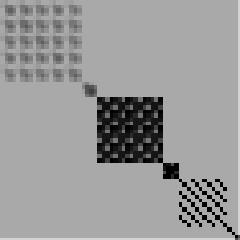
\includegraphics[scale=0.66]{figures/logo.pdf}};
\end{tikzpicture}
\end{center}

\vfill

\begin{abstract}
  Kronecker-factored approximate curvature \citep[KFAC,][]{martens2015optimizing} is arguably one of the most prominent curvature approximations in deep learning.
  Its applications range from optimization to Bayesian deep learning, training data attribution with influence functions, and model compression or merging.
  While the intuition behind KFAC is easy to understand, its implementation is tedious: It comes in many flavours, has common pitfalls when translating the math to code, and is challenging to test, which complicates ensuring a properly functioning implementation.
  Some of the authors themselves have dealt with these challenges and experienced the discomfort of not being able to fully test their code.
  Thanks to recent advances in understanding KFAC, we are now able to provide test cases and a recipe for a reliable KFAC implementation.
  \emph{This tutorial is meant as a ground-up introduction to KFAC.}
  In contrast to the existing work, our focus lies on providing both math and code side-by-side, and providing test cases based on latest insights into KFAC that are scattered throughout the literature.
  We hope this tutorial provides a contemporary view onto KFAC that
  allows beginners to gain a deeper understanding of this curvature approximation, while lowering the barrier to its implementation, extension, and usage in practise.
\end{abstract}

\vfill

\paragraph{Version:} \today\,(v1.0.0)

\paragraph{About the length of this document.}
Before you close this document because you saw the page count:
the \emph{effective length is much shorter than suggested by its page number}.
This is because \emph{we use an experimental two-column layout which presents text and code in parallel} and leads to a large amount of white space.
The left column contains the main text with explanations and mathematical descriptions.
The right column accompanies the left one with code snippets to make the ideas precise in code; it can safely be skipped if you are in a rush.
And if you already know the basics, it suffices to read the KFAC-specific part (pages \pageref{sec:kfac-overview}--\pageref{sec:kfac-cheatsheet}).

\paragraph{Follow along in code.} The \LaTeX\,\& Python source code is available at \href{\repourl}{\texttt{github.com/f-dangel/kfac-tutorial}}.
This allows you to run the code as you read:
Clone the repository and follow the installation instructions.
You can then run each snippet from the repository root, for instance by calling \texttt{python kfs/basics/forward\_pass.py}.
If you find typos or have suggestions for improving improving explanations, math, or code, please open issues and pull requests.
In doing so, you are contributing to making this tutorial a valuable reference for newcomers.

\vspace{\baselineskip}
%%% Local Variables:
%%% mode: latex
%%% TeX-master: "../main"
%%% End:
